\documentclass[10pt,letterpaper]{article}

\usepackage[margin=0.75in]{geometry}
\usepackage{tikz}

\begin{document}

  \title{CS 321, Assignment 5}
  \author{Cody Malick\\
  \texttt{malickc@oregonstate.edu}}
  \date{\today}
  \maketitle

\section{}
\subsection*{a}
	Step 1:\\
	Adversary picks $p$\\
	Step 2:\\
	I select $w=(aa)^p (bbb)^p$, where $|w| \ge p$, and $w \in A$ and $w \in
	$ real numbers\\
	Step 3:\\
	Split into $w=xyz$ where $|xy| \le p$, and $|y|>0$ \\
	Step 4:\\
	I pick $i=0$, I win if $xy^iz \notin A$\\
	Then $xy^0z=xz=(aa)^{p-|y|}(bbb)^0 \notin A$ since $|y|>0$\\
	The numbers of $num(aa,w) \ne num(bbb,w)$\\
	I win, A is not regular. 
\subsection*{b}
	Step 1:\\
	Adversary picks $p$\\
	Step 2:\\
	I select $|w|=p^2$, where $|w| \ge p$, and $w \in A$ and $w \in
	$ real numbers\\
	Step 3:\\
	Split into $w=xyz$ where $|xy| \le p$, and $|y|>0$ \\
	Step 4:\\
	I pick $i=p-1$, I win if $xy^iz \notin A$\\
	Then $xy^{p-1}z, |w|=(p+y^i)+(p-1)p < (p+1)^2 \notin A$ since $|y|>0$\\
	The length of w is not square\\
	I win, A is not regular. 
\section{}
\subsection*{a}
	$S \rightarrow 1S0\ |\ 0S1\ |\ \epsilon$
\subsection*{b}
	$S \rightarrow aST\ |\ STa\ |\ aTS\ |\ TSa\ |\ aT\ |\ Ta\ |\ \epsilon $\\
	$T \rightarrow bS\ |\ Sb\ |\ b$
\section{}
	% nEARLY Identical to the one in the video
 \begin{center}
	 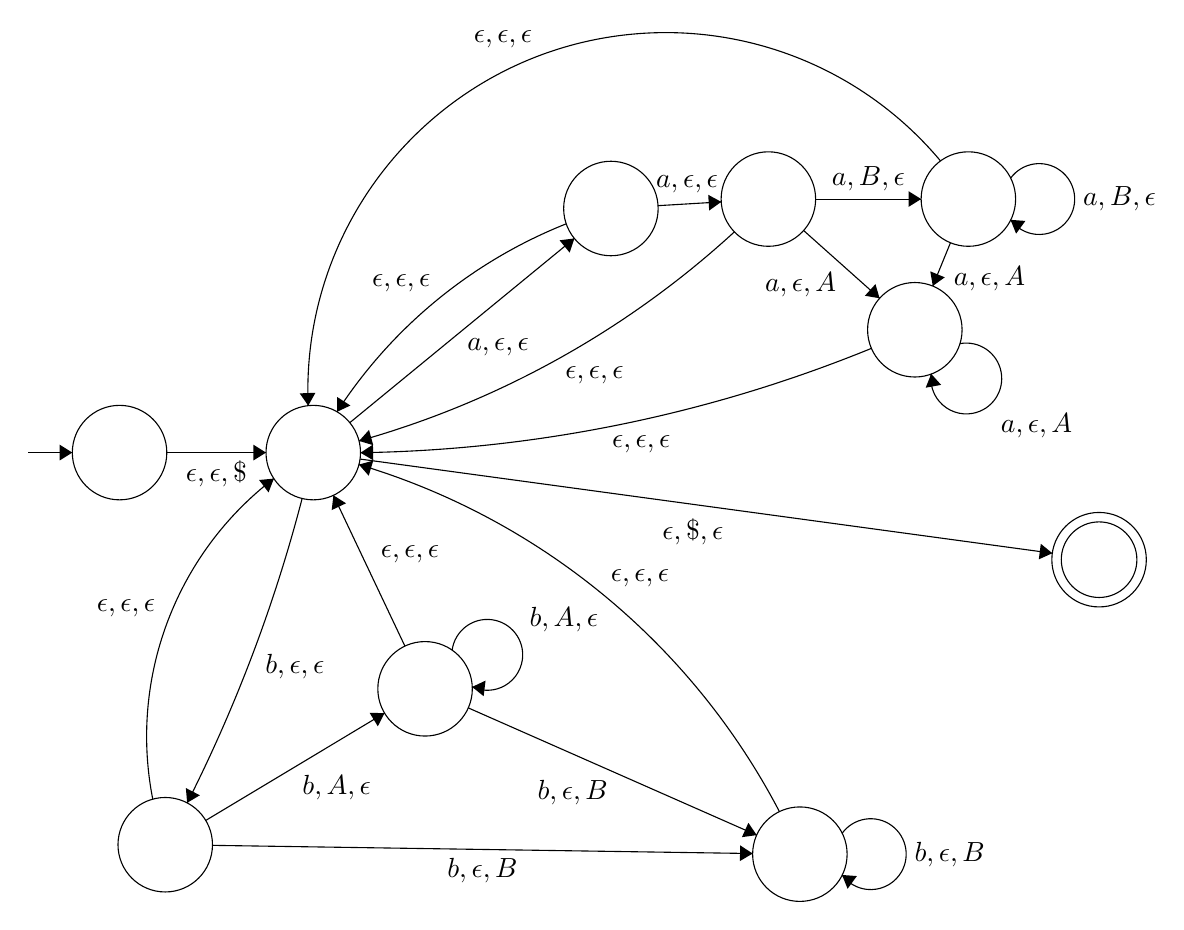
\begin{tikzpicture}[scale=0.2]
		 \tikzstyle{every node}+=[inner sep=0pt]
		 \draw [black] (8.3,-29.8) circle (3);
		 \draw [black] (20.6,-29.8) circle (3);
		 \draw [black] (39.5,-14.3) circle (3);
		 \draw [black] (49.5,-13.7) circle (3);
		 \draw [black] (58.8,-22) circle (3);
		 \draw [black] (62.2,-13.7) circle (3);
		 \draw [black] (11.2,-54.7) circle (3);
		 \draw [black] (51.5,-55.3) circle (3);
		 \draw [black] (27.7,-44.8) circle (3);
		 \draw [black] (70.5,-36.6) circle (3);
		 \draw [black] (70.5,-36.6) circle (2.4);
		 \draw [black] (2.5,-29.8) -- (5.3,-29.8);
		 \fill [black] (5.3,-29.8) -- (4.5,-29.3) -- (4.5,-30.3);
		 \draw [black] (11.3,-29.8) -- (17.6,-29.8);
		 \fill [black] (17.6,-29.8) -- (16.8,-29.3) -- (16.8,-30.3);
		 \draw (14.45,-30.3) node [below] {$\epsilon,\epsilon,\$$};
		 \draw [black] (22.92,-27.9) -- (37.18,-16.2);
		 \fill [black] (37.18,-16.2) -- (36.24,-16.32) -- (36.88,-17.1);
		 \draw (32.34,-22.54) node [below] {$a,\epsilon,\epsilon$};
		 \draw [black] (42.49,-14.12) -- (46.51,-13.88);
		 \fill [black] (46.51,-13.88) -- (45.68,-13.43) -- (45.74,-14.43);
		 \draw (44.33,-13.37) node [above] {$a,\epsilon,\epsilon$};
		 \draw [black] (51.74,-15.7) -- (56.56,-20);
		 \fill [black] (56.56,-20) -- (56.3,-19.1) -- (55.63,-19.84);
		 \draw (51.55,-18.34) node [below] {$a,\epsilon,A$};
		 \draw [black] (61.655,-22.883) arc (100.55269:-187.44731:2.25);
		 \draw (64.23,-28.11) node [right] {$a,\epsilon,A$};
		 \fill [black] (59.84,-24.8) -- (59.49,-25.68) -- (60.47,-25.5);
		 \draw [black] (52.5,-13.7) -- (59.2,-13.7);
		 \fill [black] (59.2,-13.7) -- (58.4,-13.2) -- (58.4,-14.2);
		 \draw (55.85,-13.2) node [above] {$a,B,\epsilon$};
		 \draw [black] (61.06,-16.48) -- (59.94,-19.22);
		 \fill [black] (59.94,-19.22) -- (60.7,-18.67) -- (59.78,-18.29);
		 \draw (61.24,-18.76) node [right] {$a,\epsilon,A$};
		 \draw [black] (64.88,-12.377) arc (144:-144:2.25);
		 \draw (69.45,-13.7) node [right] {$a,B,\epsilon$};
		 \fill [black] (64.88,-15.02) -- (65.23,-15.9) -- (65.82,-15.09);
		 \draw [black] (14.2,-54.74) -- (48.5,-55.26);
		 \fill [black] (48.5,-55.26) -- (47.71,-54.74) -- (47.69,-55.74);
		 \draw (31.34,-55.54) node [below] {$b,\epsilon,B$};
		 \draw [black] (54.18,-53.977) arc (144:-144:2.25);
		 \draw (58.75,-55.3) node [right] {$b,\epsilon,B$};
		 \fill [black] (54.18,-56.62) -- (54.53,-57.5) -- (55.12,-56.69);
		 \draw [black] (30.44,-46.01) -- (48.76,-54.09);
		 \fill [black] (48.76,-54.09) -- (48.23,-53.31) -- (47.82,-54.22);
		 \draw (37.07,-50.58) node [below] {$b,\epsilon,B$};
		 \draw [black] (13.77,-53.16) -- (25.13,-46.34);
		 \fill [black] (25.13,-46.34) -- (24.18,-46.33) -- (24.7,-47.18);
		 \draw (22.09,-50.25) node [below] {$b,A,\epsilon$};
		 \draw [black] (29.418,-42.355) arc (172.63909:-115.36091:2.25);
		 \draw (34.3,-40.38) node [right] {$b,A,\epsilon$};
		 \fill [black] (30.69,-44.68) -- (31.42,-45.27) -- (31.54,-44.28);
		 \draw [black] (19.892,-32.715) arc (-14.54432:-26.81973:96.618);
		 \fill [black] (12.59,-52.04) -- (13.4,-51.56) -- (12.51,-51.1);
		 \draw (17.52,-43.4) node [right] {$b,\epsilon,\epsilon$};
		 \draw [black] (22.109,-27.208) arc (147.02012:111.69064:31.015);
		 \fill [black] (22.11,-27.21) -- (22.96,-26.81) -- (22.12,-26.27);
		 \draw (26.19,-19.62) node [above] {$\epsilon,\epsilon,\epsilon$};
		 \draw [black] (47.342,-15.783) arc (-47.46995:-74.28627:58.83);
		 \fill [black] (23.51,-29.06) -- (24.41,-29.33) -- (24.14,-28.36);
		 \draw (38.46,-24.33) node [below] {$\epsilon,\epsilon,\epsilon$};
		 \draw [black] (56.043,-23.181) arc (-67.76942:-89.14958:89.253);
		 \fill [black] (23.6,-29.81) -- (24.41,-30.29) -- (24.39,-29.29);
		 \draw (41.43,-28.71) node [below] {$\epsilon,\epsilon,\epsilon$};
		 \draw [black] (20.277,-26.82) arc (-177.58691:-320.0983:22.735);
		 \fill [black] (20.28,-26.82) -- (20.74,-26) -- (19.74,-26.04);
		 \draw (32.65,-4.11) node [above] {$\epsilon,\epsilon,\epsilon$};
		 \draw [black] (23.57,-30.21) -- (67.53,-36.19);
		 \fill [black] (67.53,-36.19) -- (66.8,-35.59) -- (66.67,-36.58);
		 \draw (44.71,-33.94) node [below] {$\epsilon,\$,\epsilon$};
		 \draw [black] (26.42,-42.09) -- (21.88,-32.51);
		 \fill [black] (21.88,-32.51) -- (21.77,-33.45) -- (22.68,-33.02);
		 \draw (24.86,-36.25) node [right] {$\epsilon,\epsilon,\epsilon$};
		 \draw [black] (10.408,-51.809) arc (-168.84083:-232.52322:20.629);
		 \fill [black] (18.1,-31.45) -- (17.16,-31.54) -- (17.76,-32.33);
		 \draw (10.59,-39.71) node [left] {$\epsilon,\epsilon,\epsilon$};
		 \draw [black] (23.501,-30.562) arc (73.34776:27.59043:44.521);
		 \fill [black] (23.5,-30.56) -- (24.12,-31.27) -- (24.41,-30.31);
		 \draw (41.35,-38.38) node [above] {$\epsilon,\epsilon,\epsilon$};
	 \end{tikzpicture}
 \end{center}
\end{document}
